\documentclass[fleqn]{beamer}\usepackage[]{graphicx}\usepackage[]{color}
% maxwidth is the original width if it is less than linewidth
% otherwise use linewidth (to make sure the graphics do not exceed the margin)
\makeatletter
\def\maxwidth{ %
  \ifdim\Gin@nat@width>\linewidth
    \linewidth
  \else
    \Gin@nat@width
  \fi
}
\makeatother

\definecolor{fgcolor}{rgb}{0.345, 0.345, 0.345}
\newcommand{\hlnum}[1]{\textcolor[rgb]{0.686,0.059,0.569}{#1}}%
\newcommand{\hlstr}[1]{\textcolor[rgb]{0.192,0.494,0.8}{#1}}%
\newcommand{\hlcom}[1]{\textcolor[rgb]{0.678,0.584,0.686}{\textit{#1}}}%
\newcommand{\hlopt}[1]{\textcolor[rgb]{0,0,0}{#1}}%
\newcommand{\hlstd}[1]{\textcolor[rgb]{0.345,0.345,0.345}{#1}}%
\newcommand{\hlkwa}[1]{\textcolor[rgb]{0.161,0.373,0.58}{\textbf{#1}}}%
\newcommand{\hlkwb}[1]{\textcolor[rgb]{0.69,0.353,0.396}{#1}}%
\newcommand{\hlkwc}[1]{\textcolor[rgb]{0.333,0.667,0.333}{#1}}%
\newcommand{\hlkwd}[1]{\textcolor[rgb]{0.737,0.353,0.396}{\textbf{#1}}}%
\let\hlipl\hlkwb

\usepackage{framed}
\makeatletter
\newenvironment{kframe}{%
 \def\at@end@of@kframe{}%
 \ifinner\ifhmode%
  \def\at@end@of@kframe{\end{minipage}}%
  \begin{minipage}{\columnwidth}%
 \fi\fi%
 \def\FrameCommand##1{\hskip\@totalleftmargin \hskip-\fboxsep
 \colorbox{shadecolor}{##1}\hskip-\fboxsep
     % There is no \\@totalrightmargin, so:
     \hskip-\linewidth \hskip-\@totalleftmargin \hskip\columnwidth}%
 \MakeFramed {\advance\hsize-\width
   \@totalleftmargin\z@ \linewidth\hsize
   \@setminipage}}%
 {\par\unskip\endMakeFramed%
 \at@end@of@kframe}
\makeatother

\definecolor{shadecolor}{rgb}{.97, .97, .97}
\definecolor{messagecolor}{rgb}{0, 0, 0}
\definecolor{warningcolor}{rgb}{1, 0, 1}
\definecolor{errorcolor}{rgb}{1, 0, 0}
\newenvironment{knitrout}{}{} % an empty environment to be redefined in TeX

\usepackage{alltt}

\mode<presentation>
%\usetheme{Frankfurt}
\usetheme{boxes}
\usecolortheme{beaver}
%\usetheme{Singapore}
%\usetheme{Hannover}

%%%%%%%%%%%%%%%%%%%%%
% Estimating Economic Costs
%%%%%%%%%%%%%%%%%%%%%
\IfFileExists{upquote.sty}{\usepackage{upquote}}{}
\begin{document}




%===================================
% Logistics
%===================================
\title{AECN 896-003}
\author{Taro Mieno}
\everymath{\displaystyle}

\begin{frame}
\titlepage
\end{frame}

\begin{frame}[c,fragile]
  \frametitle{Instructors}
  \begin{block}{Instructor}
    Taro Mieno (Office: 209, E-mail: tmieno2@unl.edu)
  \end{block}
  \begin{block}{Teaching Assistant}
    Shunkei Kakimoto (E-mail: skakimoto3@huskers.unl.edu)
  \end{block}
\end{frame}

%----------------- end of frame -----------------%

\begin{frame}[c,fragile]
  \frametitle{Goals of the course}
  \begin{itemize}
    \item Learn modern introductory econometric theory
    \item Apply econometric theories to real economic problems
    \item Learn how to use statistical software (R) so you can conduct research independently (without technical help from your advisor)
    \begin{itemize}
      \item manage data
      \item visualize data
      \item run regressions
      \item interpret results
    \end{itemize}
  \end{itemize}
\end{frame}

\begin{frame}[c]
  \frametitle{Text Books}
  \begin{block}{Required:}
    Wooldridge, Jeffrey M. 2006. ``Introductory Econometrics: A Modern Approach (\textcolor{red}{5}th edition).'' Mason, OH: Thomson/South-Western.
  \end{block}
  \begin{block}{Recommended:}
  \begin{itemize}
    \item Florian, Heiss. 2016 ``Using R for Introductory Econometrics.'' CreateSpace Independent Publishing Platform. (free version available online \href{http://www.urfie.net/}{\underline{here}})
    \item Norman, Matloff. 2011 ``The Art of R Programming: A Tour of Statistical Software Design.'' No Starch Press. (\href{https://www.amazon.com/Art-Programming-Statistical-Software-Design/dp/1593273843}{link to the book on Amazon})
  \end{itemize}
  \end{block}
\end{frame}


%----------------- end of frame -----------------%

\begin{frame}[c,fragile]
\begin{block}{Course Schedule}
  \begin{itemize}
    \item Lectures (MW), 3:00-4:30pm: by me
    \item Lab sessions (F), 1:00-2:30pm: led by me and Shunkei
  \end{itemize}
\end{block}

  \begin{block}{Note:}
    I frequently use $R$ within lectures. You are advised to bring your laptop to every class if you want to get the most out of each lecture.
  \end{block}
\end{frame}

%----------------- end of frame -----------------%

\begin{frame}[c,fragile]
  \frametitle{Grading}
\begin{center}
\begin{tabular}{lc}
   Problem sets (4 assignments) :& 50\% \\
   Paper: & 50\%\\
     $\;\;\;\;$ Proposal: & 5\%\\
     $\;\;\;\;$ Final paper: & 45\%\\\hline
   Total: & 100\%
\end{tabular}
\end{center}
\end{frame}

\begin{frame}[c]
  \frametitle{Assignments}
  \begin{block}{Problem sets}
    \begin{itemize}
    \item Most questions are from the required text book
    \item Some questions come from what we cover in lab sessions
    \end{itemize}
  \end{block}
  \begin{block}{Rmarkdown to do and submit your problem sets}
  \begin{itemize}
    \item You are required to present your R program
    \item You learn how to compile your assignment with your R code written in a document using \textcolor{red}{Rmarkdown}, which will be covered in the second lab session
  \end{itemize}
  \end{block}
\end{frame}

\begin{frame}[c]
  \frametitle{Assignments}
  \begin{block}{Caution}
    \begin{itemize}
      \item 2nd year students have answers to all the questions I will assign (I will use exactly the same problems because they are really good to learn econometrics)
      \item You are free to copy and paste (or rephrase) the answers for your assignment. I won't bother to try to tell if you have copied and pasted answers.
      \only<3->{\item However, you are simply doing dis-service to yourself by depriving yourself of learning opporunities}
      \only<4->{\item Moreover, your lack of understanding of the material will be clearly manifested on your final paper (I am not at all shy of giving bad grades on the final paper)}
    \end{itemize}
  \end{block}
\end{frame}

\begin{frame}[c]
  \frametitle{Paper}
  In this assignment,
  \begin{itemize}
    \item you write 
    \begin{itemize}
      \item a paper proposal with in-class presentation (5 points)
      \item a paper with a particular emphasis on econometric analysis using a real world data set (45 points)
    \end{itemize}
    \item you are encouraged to use the data set you are using for your masters thesis (talk with your advisor)
    \item you need to ensure that you use a \textcolor{red}{panel} dataset
    \item No presentation of your final paper
  \end{itemize}
\end{frame}

\begin{frame}[c]
  \frametitle{Paper}
  Here is the time line of the paper assignment:
  \begin{itemize}
    \item \textcolor{blue}{Oct, 7}: identify a research topic and the data set you will be using, and get an approval from the instructor
    \item \textcolor{blue}{Oct, 21}: paper proposal and presentation
    \item \textcolor{blue}{Dec, 9}: final paper 
  \end{itemize}
\end{frame}

\begin{frame}[t]
  \frametitle{Paper Proposal} 
  \begin{block}{Introduction}
    \begin{enumerate}
      \item clear identification of what you are trying to find out (research question) 
      \item why the research question is worthwhile answering 
    \end{enumerate}
  \end{block}
  \begin{block}{Simple Model}  
    \begin{itemize}
      \item dependent variable (the variable to be explained)
      \item explanatory variable (variables to be explain)
    \end{itemize}
  \end{block}
  \begin{block}{Data Source}
     \begin{enumerate}
      \item where you get data
    \end{enumerate}
  \end{block}
\end{frame}

\begin{frame}[t]
  \frametitle{Final Paper}
  \begin{block}{Introduction}
    \begin{enumerate}
      \item clear identification of what you are trying to find out (research question) [1 point]
      \item why the research question is worthwhile answering [1 point]
    \end{enumerate}
  \end{block}
  \begin{block}{Data description}
     \begin{enumerate}
      \item the nature of the data with summary statistics table [1 point]
      \item visualize a few key variables in a meaningful way [3 points]
    \end{enumerate}
  \end{block}
\end{frame}

\begin{frame}[c]
  \frametitle{Final Paper}
  \begin{block}{Econometric Methods:}
    the \textcolor{blue}{process} of how you end up with the final econometric models and methods. [40 points (\textcolor{blue}{or more})]
    \begin{enumerate}
      \item justification of your choice of independent variables
      \item potential endogeneity problems
      \item what did you do to address the endogeneity problems?
      \item justification of econometric model(s) and method(s)
      \item identify appropriate standard error estimation methods
    \end{enumerate}
  \end{block}
  \begin{block}{Results, Discussions, and Conclusions:}
    \begin{enumerate}
        \item interpret and describe the results [2 points]
        \item implications of the results [1 point]
        \item conclusions [1 point]
     \end{enumerate}
  \end{block}
\end{frame}
%----------------- end of frame -----------------%

%===================================
% Lecture
%===================================
\title{What is econometrics about?}
\author{}
\date{}
\everymath{\displaystyle}

\begin{frame}
\titlepage
\end{frame}

\begin{frame}[c]
  \frametitle{What econometrics is about}
  \begin{block}{Econometrics}
     Estimate quantitative relationships between variables
  \end{block}
  \begin{block}{Examples:}
    \begin{itemize}
      \item the impact of fertilizer on crop yield
      \item the impact of political campaign expenditure on voting outcomes
      \item the impact of education on wage
    \end{itemize}
  \end{block}
\end{frame}


\begin{frame}[c]
  \frametitle{Steps in Econometric Analysis}
  \begin{enumerate}
     \item formulation of the question of interest (what are you trying to find out?)
     \item develop an economic model of the phenomenon you are interested in understanding (identify variables that matter)
     \item turn the economic model into an econometric model
     \item collect data
     \item \textcolor{blue}{estimate the model using econometrics}
     \item \textcolor{blue}{test hypotheses}
  \end{enumerate}
\end{frame}

\begin{frame}[c]
  \frametitle{Step 2: Develop an economic model}
  \begin{block}{Job training and worker productivity}
  \vspace{-0.6cm}
  \begin{align}
     wage = f(educ,exper,training) \notag
  \end{align}
  \begin{itemize}
    \item $wage$: hourly wage
    \item $educ$: years of formal education
    \item $exper$: years of workforce experience
    \item $training$: weeks spent in job training
  \end{itemize}
  \end{block}
  (Depending on questions you would like to answer, the economic model can be much more involved)
\end{frame}

\begin{frame}[c]
  \frametitle{Step 3: Develop an econometric model}

  \begin{block}{Job training and worker productivity}
  \vspace{-0.6cm}
  \begin{align}
     wage = f(educ,exper,training) \notag
  \end{align}
  The form of the function $f(\cdot)$ must be specified (almost always) before we can undertake an econometric analysis
  \begin{align}
     wage = \beta_0 + \beta_1 educ + \beta_2 exper + \beta_3 training + u \notag
  \end{align}

  \end{block}

\end{frame}

\begin{frame}[c]
  \frametitle{Step 3: Develop an econometric model}
  \begin{block}{The econometric model}
  \vspace{-0.6cm}
     \begin{align}
     wage = \beta_0 + \beta_1 educ + \beta_2 exper + \beta_3 training + u \notag
     \end{align}
  \end{block}
  \begin{block}{$\theta=\{\beta_0,\beta_1,\beta_2,\beta_3\}$}
    \begin{itemize}
    \item are the \textcolor{blue}{parameters} of the econometric model.
    \item describe the directions and strengths of the relationship between $wage$ and the factors used to determine $wage$ in the model
    \end{itemize}
  \end{block}
  \begin{block}{$u$}
    \begin{itemize}
      \item is called error term
      \item includes \textcolor{red}{ALL} the other factors that can affect wage other than the included variables (like innate ability)
    \end{itemize}
  \end{block}
\end{frame}

\begin{frame}[c]
  \frametitle{Step 4: Collect data}
  \begin{itemize}
     \item survey
     \item websites
     \item experiment
  \end{itemize}
\end{frame}

\begin{frame}[c]
  \frametitle{Data types}
  \begin{block}{Cross-sectional Data}
  \begin{itemize}
    \item a sample of individuals, households, firms, cities, states, countries, or a variety of other units, taken at a given point in time
    \item the data on all units do not correspond to precisely the same time period
      \begin{itemize}
        \item some families surveyed during different weeks within a year
      \end{itemize}
  \end{itemize}
  \end{block}
\end{frame}

\begin{frame}[c,fragile]
  \frametitle{Cross-sectional Data}

\begin{knitrout}
\definecolor{shadecolor}{rgb}{0.969, 0.969, 0.969}\color{fgcolor}\begin{kframe}
\begin{verbatim}
      wage educ exper female married
  1:  3.10   11     2      1       0
  2:  3.24   12    22      1       1
  3:  3.00   11     2      0       0
  4:  6.00    8    44      0       1
  5:  5.30   12     7      0       1
 ---                                
522: 15.00   16    14      1       1
523:  2.27   10     2      1       0
524:  4.67   15    13      0       1
525: 11.56   16     5      0       1
526:  3.50   14     5      1       0
\end{verbatim}
\end{kframe}
\end{knitrout}

\end{frame}

\begin{frame}[c]
  \frametitle{Data types}
  \begin{block}{Time-series Data}
    Observations on a variable or several variables over time
  \end{block}
  \begin{block}{Examples}
    \begin{itemize}
      \item corn price
      \item oil price
    \end{itemize}
  \end{block}
  \begin{itemize}
    \item The econometric frameworks necessary to analyze time series data are quite different from those for cross-sectional data
    \item We do \textcolor{red}{NOT} learn time-series econometric methods
  \end{itemize}
\end{frame}

\begin{frame}[c]
  \frametitle{Data types}
  \begin{block}{Panel (Longitudinal) Data}
    time series for each cross-sectional member in the data set (\textcolor{blue}{same} cross-sectional units are tracked over a given period of time)
  \end{block}
  \begin{block}{Examples}
    \begin{itemize}
      \item wage data for individuals collected every five years over the past 30 years
      \item yearly GDP data for 60 countries over the past 10 years
    \end{itemize}
  \end{block}
  \begin{block}{Notes}
    \begin{itemize}
     \item Panel data are much more common than they used to be
     \item Panel data econometric methods take advantage of the panel data structure
  \end{itemize}
  \end{block}
\end{frame}

\begin{frame}[c,fragile]
  \frametitle{Panel (Longitudinal) Data}
\begin{knitrout}
\definecolor{shadecolor}{rgb}{0.969, 0.969, 0.969}\color{fgcolor}\begin{kframe}
\begin{verbatim}
     county year    crmrte   prbarr  prbpris
  1:      1   81 0.0398849 0.289696 0.472222
  2:      1   82 0.0383449 0.338111 0.506993
  3:      1   83 0.0303048 0.330449 0.479705
  4:      1   84 0.0347259 0.362525 0.520104
  5:      1   85 0.0365730 0.325395 0.497059
 ---                                        
626:    197   83 0.0155747 0.226667 0.428571
627:    197   84 0.0136619 0.204188 0.372727
628:    197   85 0.0130857 0.180556 0.333333
629:    197   86 0.0128740 0.112676 0.244444
630:    197   87 0.0141928 0.207595 0.360825
\end{verbatim}
\end{kframe}
\end{knitrout}
\end{frame}

\begin{frame}[c]
  \frametitle{Step 5 and 6}
  This is what you learn for the next few months!!
  \begin{itemize}
    \item estiamte the model using econometrics
    \item test hypothesis
  \end{itemize}
\end{frame}

\title{Causality and Association}
\author{}
\date{}

\begin{frame}
\maketitle
\end{frame}

\begin{frame}[t]
  \frametitle{Causality and Association}
  \begin{block}{Association}
    An association of two variables arise because \textcolor{red}{either of or both} variables affect the other variable
    \begin{align}
     A \longleftrightarrow B \notag
    \end{align}
    Association does not concern which affects which. This is what \textcolor{blue}{correlation coefficient} measures.
  \end{block}

  \begin{block}{Causality}
    Causal effect is the impact of one variable on the other,
    \begin{align}
     A \rightarrow B \notag
    \end{align}
    Here, changes in $A$ cause changes in $B$
  \end{block}
\end{frame}

\begin{frame}[c]
  \frametitle{Causality and Association}
  \begin{block}{An interesting CM}
    \href{https://www.youtube.com/watch?v=KSHMgoUWBmY}{Click here for an interesting Youtube video}
  \end{block}

  \only<2->{
  \begin{block}{So, the guy is trying to convince you that}
    \begin{itemize}
      \item wear glasses $\rightarrow$ much smarter than those who don't
      \item wear glasses $\rightarrow$ more likely to pursue higher education
      \item wear glasses $\rightarrow$ 200$\%$ more likely to graduate college
    \end{itemize}

  \only<3->{
    So, wearing glasses has \textcolor{blue}{causal} positive impacts on some good qualities. Buy glasses!!
  }
  \end{block}
  }
\end{frame}

\begin{frame}[c]
  \frametitle{Causality and Association}
  \begin{block}{But, isn't this more like the true mechanism?}
    nerd $\rightarrow$ \textcolor{blue}{more time studying} $\rightarrow$ much smarter (knowledgeable), more likely to pursue higher education and graduate college, and wear glasses
  \end{block}

  \begin{block}{So,}
    Wearing glasses are \textcolor{blue}{associated} with the good qualities, but do not cause them
  \end{block}

\end{frame}

\begin{frame}[c]
  \frametitle{Causal Effect}
  Almost always, we care about isolating causal effects, but not association
  \begin{itemize}
    \item wear glasses $\rightarrow$ smart
    \item education $\rightarrow$ income
    \item nitrogen $\rightarrow$ yield
  \end{itemize}
\end{frame}


\title{Endogeneity: Your Nemesis}
\author{}
\date{}

\begin{frame}
\maketitle
\end{frame}

\begin{frame}[c]
  \frametitle{Causality and Association}
  \begin{block}{Causality and Association}
    It is super easy to find an association of multiple variables, but it is incredibly hard to find a causal effect (at least in Economics)!!
  \end{block}
\end{frame}

\begin{frame}[c]
  \frametitle{Endogeneity}
  \only<1-1>{\begin{block}{You are interested in}
    the causal impact of fire fighters on the number of death tolls in fire events
  \end{block}}

  \begin{block}{The (Fake) Data}
  \begin{center}
  \begin{tabular}{ c c c }
  Fire event & death toll & \# of fire fighters \\\hline
    1 & 10 & 20 \\
    2 & 0 & 3 \\
    3 & 5 & 10 \\
    4 & 3 & 5 \\
    5 & 50 & 50 \\
  \end{tabular}
  \end{center}

  \end{block}

  \only<2-2>{\begin{block}{Questions}
    \begin{itemize}
      \item How are they associated?
      \item Can you say anything about the causal effect of fire fighters deployment on the number of death tolls?
    \end{itemize}
  \end{block}}
\end{frame}

\begin{frame}[c]
  \frametitle{Causality and Association}
\begin{center}
\begin{block}{What happened?}
  \only<2->{You ignored an important variable!!\\\vspace{0.6cm}

  \begin{tabular}{cccc}
    Fire event & death toll & \# of fire fighters & scale \\\hline
    1 & 10 & 20 & 40\\
    2 & 0 & 3 & 5\\
    3 & 5 & 10 & 20\\
    4 & 3 & 5 & 10\\
    5 & 50 & 50 & 100\\
  \end{tabular}}

\end{block}

\end{center}

\end{frame}


\begin{frame}[c]
  \frametitle{Endogeneity Problem}
  \begin{block}{\textcolor{blue}{Endogeneity Problem}}
    Variables of interest are correlated with some unobservables (variables that cannot be observed or are missing) that have non-zero impacts on the variable that you want to explain
  \end{block}
\end{frame}

\begin{frame}[c]
  \begin{block}{In the above example,}
    \begin{description}[variable of interest]
      \item [variable of interest]: the number of firefighters
      \item [unobservables]: the scale of fire events (and other factors)
      \item [variable to explain]: death toll
    \end{description}
  \end{block}

  \begin{block}{The model}
    \begin{align*}
      \mbox{death toll} = \alpha + \beta\; \mbox{\# of fire fighters} + (\gamma\; \mbox{scale} + v)
    \end{align*}
  \end{block}

  \begin{block}{Endogeneity Problem}  
    \# of fire fighters is correlated with scale, which we ignored
  \end{block}

\end{frame}

\begin{frame}[c]
  \frametitle{Endogeneity Problem}
  \begin{block}{Another example: education on wage}
    \begin{align*}
    wage = \beta_0 + \beta_1 educ + \beta_2 exper + \beta_3 training + u \notag
    \end{align*}
    \begin{itemize}
      \item What are unobservables in $u$ that are likely to be correlated with $educ$?
    \end{itemize}
  \end{block}
  \only<2-2>{\begin{block}{An important unobservable}
    \begin{itemize}
      \item innate ability $\rightarrow$ wage
      \item innate ability $\rightarrow$ education
    \end{itemize}
  \end{block}}
\end{frame}

\begin{frame}[c]
  \frametitle{Endogeneity Problem}
  \begin{block}{Many sources of endogeneity problems}
  Most of the time, you will be faced with endogeneity problems caused by at least one of the followings,
  \begin{itemize}
    \item omitted variables (the scale of fire events, innate ability)
    \item self-selection
    \item simultaneity
    \item measurement error
  \end{itemize}
  \textcolor{blue}{A lot more on this later.}
  \end{block}
  \begin{block}{Central question}
    How can we avoid or solve endogneity problems?
  \end{block}
\end{frame}

\begin{frame}[c]
  \frametitle{How to deal with endogeneity?}
  \begin{itemize}
    \item You have two opportunities to deal with endogeneity problems
  \begin{itemize}
    \item at the design stage
    \item at the regression stage (what you will learn in this course)
  \end{itemize}
  \only<2->{\item Econometrics has evolved to address endogeneity problems at the regression stage because randomized experiments are infeasible most of the time}
  \only<3->{\item How about econometrics and other fields of statistics: Statistics, Psychometrics, and Biometrics?
  \begin{center}
  \begin{tabular}{ccc}
  Field & Design & Estimation Method \\
  \hline
  Econometrics & not feasible (often) & intricate \\
  Many other fields & feasible & relatively simple \\\\
  \end{tabular}
  \end{center}}

  \end{itemize}
\end{frame}


\begin{frame}[c]
  \frametitle{Deal with endogneity}
  \begin{block}{Randomized Experiments}
    \begin{itemize}
      \item you have a liberty to determine the level of the variable of interest
      \item by randomizing the value of the variable of interest, you can effectively break the link (association) with whatever is included in the error term
    \end{itemize}
  \end{block}
\end{frame}

\begin{frame}[c]
  \frametitle{Randomized Experiments}
  \begin{figure}
  \centering
      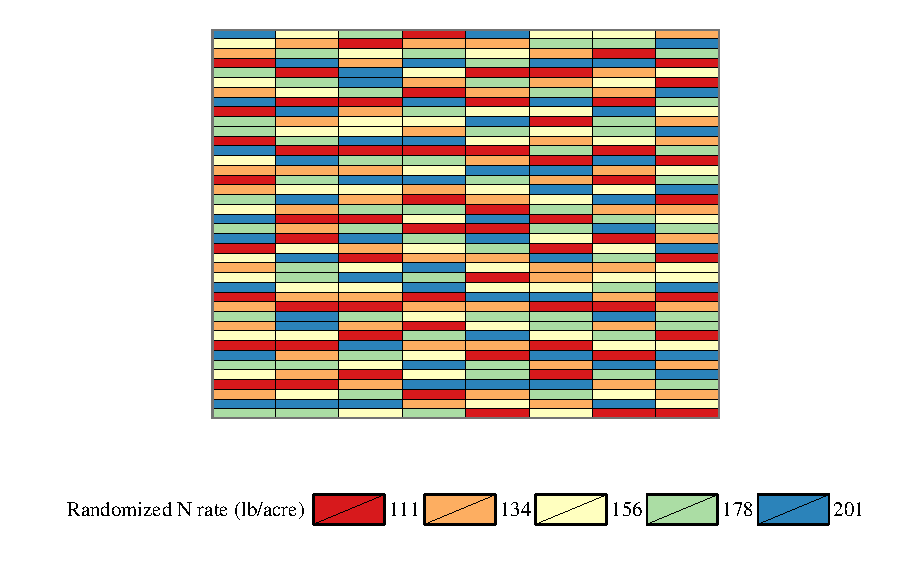
\includegraphics[trim = 0mm 0mm 0mm 0mm, clip,width=0.8\textwidth]{field_map_N_IL.pdf}
  \end{figure}
  \begin{block}{Important}
    Soil quality (in error term) is still not held fixed (moves together with N), but it is no longer correlated with N!!
  \end{block}
\end{frame}

\begin{frame}[c]
  \frametitle{Randomized Experiments on Education?}
  \begin{block}{Randomized Experiment?}
    Researchers determine randomly how much education subjects can get?
  \end{block}

  \only<2-2>{\begin{block}{(Most) Economic data}
     are confounded with peoples' decisions
      \begin{itemize}
        \item how much education one get is determined based on their judgment of their own ability (not by rolling a dice)
        \item how many fire fighters to be deployed was determined based on the scale of fire (not by rolling a dice)
      \end{itemize}
  \end{block}}
\end{frame}


\begin{frame}[c]
  \frametitle{Prediction vs. Causality}
\begin{block}{Prediction}
  \begin{itemize}
    \item interested in the \textcolor{red}{state} of the dependent variable predicted by the model in order to \textcolor{red}{act on} it
    \begin{itemize}
      \item commodity price
      \item forest coverage
    \end{itemize}
    \item endogeneity does not matter, but fit ($R^2$) matters
  \end{itemize}
\end{block}
\end{frame}

\end{document}

